\section*{Plan for Round 1: 07/08--07/18}

We are concerned with the complexity of adiabatic-based computation using a transverse-field Ising model (TFIM).
Typically, the model is described by the Hamiltonian
\begin{align}\label{eq:TFIM}
H = \sum_{\langle i, j \rangle} V_{ij}n_in_j -  \sum_{j} \Delta_j(t) n_j + \frac{\Omega(t)}{2} \sum_{i} X_i.   
\end{align}
Here $\Delta_j(t)$ and $\Omega(t)$ are time-dependent, while $V_{ij}$ is a time-independent matrix encoding the interaction strength between qubits $i$ and $j$.
By designing the path of $\Delta_j(t)$ and $\Omega(t)$ (see Figure~\ref{fig:sweepshape}), it is possible to solve the weighted maximum independent set (WMIS) problem encoded by
$$
H_{\rm WMIS}
=-\sum_{v\in V}\Delta_{\mathrm{final}} n_v+\sum_{(u,v)\in E}V_{uv}n_un_v,
\qquad n_v\in\{0,1\},
$$
Typically, the allowed structure of $V_{ij}$ is described by weighted unit disk graphs (UDGs)~\cite{das2020efficient}.

\begin{figure}[!htbp]
    \centering
    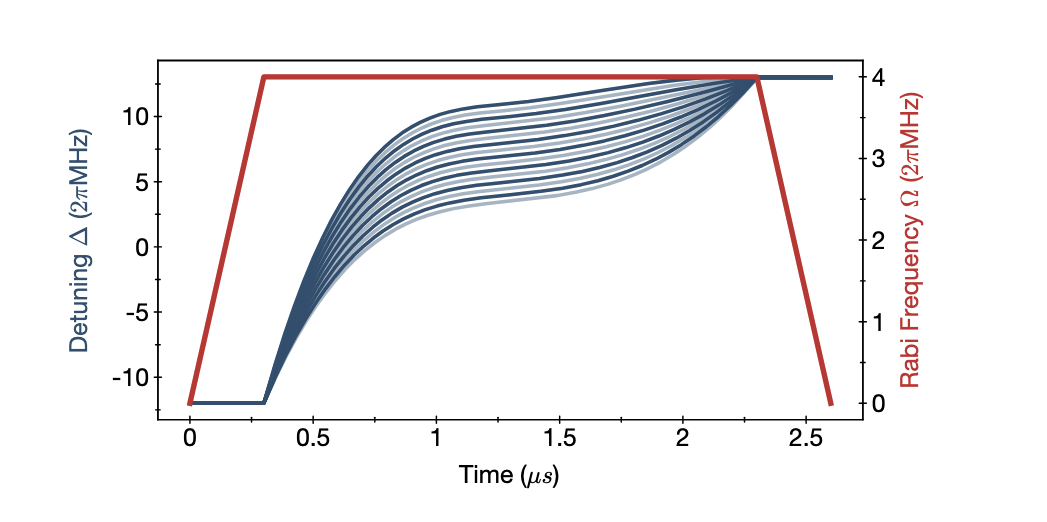
\includegraphics[width = 0.7\textwidth]{figures/sweepshape.png}
    \caption{A typical sweep of $\delta(t)$ and $\Omega(t)$ in experiment~\cite{ebadi2022quantum}}
    \label{fig:sweepshape}
\end{figure}

We ask the following general questions:

\vspace{1em}

\textbf{Q1}: This is not a typical adiabatic process of the form $(1-t)H_X + t H_Z$. How can we explain its power in solving the WMIS? How can we analyze the energy gap along the adiabatic path for different settings of $J_{ij}$?
\begin{itemize}
    \item Previous works~\cite{Amin_2009} have already shown that, under the $(1-t)H_X + t H_Z$ setting, a family of $H_Z$ has an exponentially small gap along the sweep path.
    \item \SYC{Todo: Find more references related to the energy gap analysis of Eq.~\eqref{eq:TFIM}}.
\end{itemize}

\vspace{1em}

\textbf{Q2}: Is it possible to encode a well-known quantum algorithm, which can already be represented as an adiabatic quantum computation, into a UGC-WMIS with an ensured adiabatic energy gap along the path?
\begin{itemize}
    \item In reference~\cite{nguyen2023quantum}, a general gadget is constructed to encode any WMIS or QUBO into a UGC-WMIS, but without explicit energy gap guarantees.
    \item The UGC-WMIS has a polynomial-time approximation scheme (PTAS)~\cite{das2020efficient}. Does this mean that we can at least trivially translate the PTAS into an "adiabatic quantum algorithm" to approximately solve all UGC-WMIS instances with gap guarantees?
\end{itemize}

\vspace{1em}

\textbf{Q3}: The sweep path of $\Delta(t),\Omega(t)$ is too simple. Would pulse-like design of $\Omega(t)$ and $\Delta(t)$ goes beyonds the UDG-WMIS?
\begin{itemize}
    \item A recent work realized universal quantum computation~\cite{werner2026polynomial}
    \item A recent work use echo-adiabatic precess to increase the precision of many-body state preparation~\cite{zeng2026adiabatic}
\end{itemize}

\subsection*{Todolist}

\begin{itemize}
    \item Solve Q1,  Minimum Deliverable: a note and a pre about how to analysis the adiabatic energy gap of $(1-t)H_X + t H_Z$
    \item Solve Q2, Minimum Deliverable:  a note and a pre about how to reduce problems to UGC-WMIS:
\end{itemize}

\subsection*{Idea pocket}

\begin{enumerate}
    \item Is it possible to design a randomized ising graph such that on the average case, the energy gap is exponenetially small/constant?
    \item Would multi-copy measurements benifits the adiabatic evolution gap?
\end{enumerate}
